\def\allfiles{}
\documentclass[12pt,a4paper]{article}
\usepackage{amsfonts}
\usepackage{amsmath}
\usepackage{amssymb}
\usepackage{geometry}
\usepackage{indentfirst}
\usepackage{pifont}
\usepackage{ulem}
\usepackage{color}
\usepackage{algorithm} 
\usepackage{algorithmicx} 
\usepackage{algpseudocode}  
\usepackage{amsmath}  
\usepackage{bm}
\usepackage{graphicx}
\usepackage{tcolorbox}
\renewcommand{\algorithmicrequire}{\textbf{Input:}}  % Use Input in the format of Algorithm  
\renewcommand{\algorithmicensure}{\textbf{Output:}} % Use Output in the format of Algorithm  

\setlength{\parindent}{0em}
\geometry{left=2.0cm,right=2.0cm,top=2.5cm,bottom=2.5cm}

\begin{document}
\title{Review of Recurrent Neural Network and Long Short-Term Memory Network}
\author{Guannan Hu}
\maketitle

\begin{figure}
\centering   
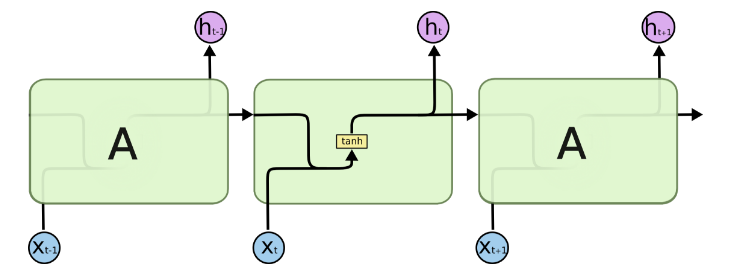
\includegraphics[width=0.5\textwidth]{pic/1.PNG}
\caption{The repeating module in a stardard RNN contains a single layer}
 \label{fig:1} 
\end{figure}



\begin{figure}
\centering   
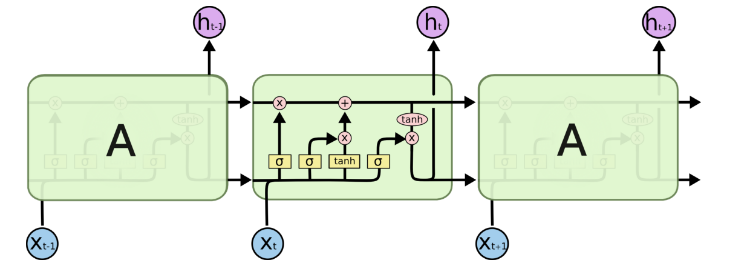
\includegraphics[width=0.5\textwidth]{pic/2.PNG}
\caption{The repeating module in an LSTM contains four interaction layers}
 \label{fig:2} 
\end{figure}

\begin{figure}[h!]
\centering   
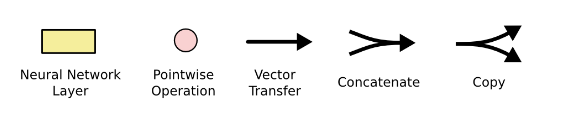
\includegraphics[width=0.5\textwidth]{pic/3.PNG}
\caption{the operations in LSTM}
 \label{fig:3} 
\end{figure}
\paragraph{} In Figure \ref{fig:3}, each line carries an entire vector, from the output of one node to the inputs of others. The pink circles represent pointwise operations, like vector addition, while the yello boxes are learned neural network layers. Lines merging denote concatenation, while a line forking denote its content being copied and the copies going to different locations.


\begin{figure}
\centering   
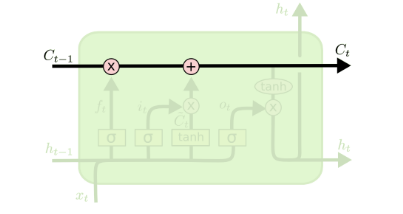
\includegraphics[width=0.4\textwidth]{pic/4.PNG}
\caption{The details of LSTM Cell}
 \label{fig:4} 
\end{figure}


\begin{figure}
\centering   
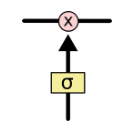
\includegraphics[width=0.2\textwidth]{pic/5.PNG}
\caption{The sigmoid layer in LSTM Cell}
 \label{fig:5} 
\end{figure}


\begin{figure}
\begin{minipage}[c]{0.5\textwidth}
\centering   
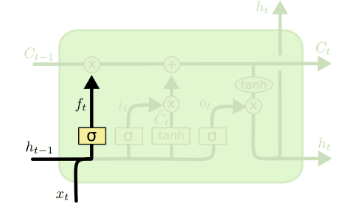
\includegraphics[width=0.8\textwidth]{pic/6.PNG}
\end{minipage}
%
\begin{minipage}[c]{0.5\textwidth}
\begin{equation*}
	\begin{array}{l}
	f_t = \delta(W_f \cdot [h_{t-1}, x_t] + b_f)
	\end{array}
\end{equation*}
\end{minipage}
\caption{The details of LSTM Cell 2}
 \label{fig:6} 
\end{figure}

\begin{figure}
\begin{minipage}[c]{0.5\textwidth}
\centering   
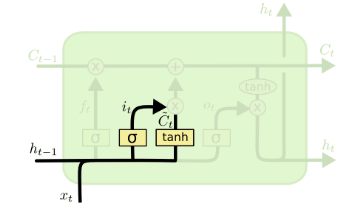
\includegraphics[width=0.8\textwidth]{pic/7.PNG}
\end{minipage}
%
\begin{minipage}[c]{0.5\textwidth}
\begin{equation*}
	\begin{array}{l}
	i_t = \delta (W_i \cdot [h_{t-1}, x_t] + b_i)\\
	\tilde{C}_t = \tanh(W_C \cdot [h_{t-1}, x_t] + b_{C})
	\end{array}
\end{equation*}
\end{minipage}
\caption{The details of LSTM Cell 3}
 \label{fig:7} 
\end{figure}

\begin{figure}
\begin{minipage}[c]{0.5\textwidth}
\centering   
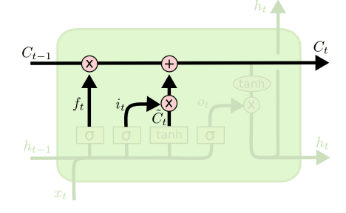
\includegraphics[width=0.8\textwidth]{pic/8.PNG}
\end{minipage}
%
\begin{minipage}[c]{0.5\textwidth}
\begin{equation*}
	\begin{array}{l}
	C_t = f_t * C_{t-1} + i_t * \tilde{C}_t
	\end{array}
\end{equation*}
\end{minipage}
\caption{The details of LSTM Cell 3}
 \label{fig:8} 
\end{figure}

\begin{figure}
\begin{minipage}[c]{0.5\textwidth}
\centering   
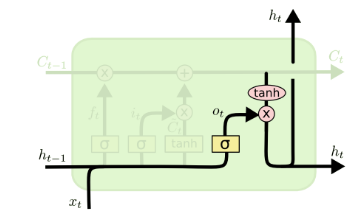
\includegraphics[width=0.8\textwidth]{pic/9.PNG}
\end{minipage}
%
\begin{minipage}[c]{0.5\textwidth}
\begin{equation*}
	\begin{array}{l}
	o_t = \delta (W_o \cdot [h_{t-1}, x_t] + b_o)\\
	h_t = o_t * \tanh(C_t)
	\end{array}
\end{equation*}
\end{minipage}
\caption{The details of LSTM Cell 4}
 \label{fig:9} 
\end{figure}

\begin{figure}
\begin{minipage}[c]{0.5\textwidth}
\centering   
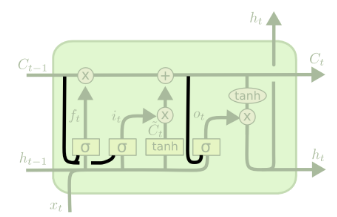
\includegraphics[width=0.8\textwidth]{pic/10.PNG}
\end{minipage}
%
\begin{minipage}[c]{0.5\textwidth}
\begin{equation*}
	\begin{array}{l}
	f_t = \delta(W_f \cdot [C_{t-1}, h_{t-1}, x_{t}] + b_f) \\
	i_t = \delta(W_{i} \cdot [C_{t-1}, h_{t-1}, x_{t}] + b_i) \\
	o_t = \delta(W_{o} \cdot [C_{t}, h_{t-1}, x_{t}] + b_{o})
	\end{array}
\end{equation*}
\end{minipage}
\caption{Variant of LSTM 1 : adding peephole connections}
 \label{fig:10} 
\end{figure}

\begin{figure}
\begin{minipage}[c]{0.5\textwidth}
\centering   
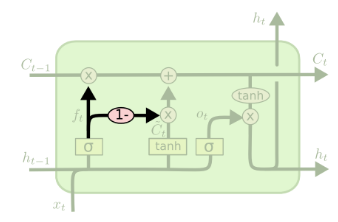
\includegraphics[width=0.8\textwidth]{pic/11.PNG}
\end{minipage}
%
\begin{minipage}[c]{0.5\textwidth}
\begin{equation*}
	C_t = f_t * C_{t-1} + (1 -f_t) * \tilde{C}_t
\end{equation*}

\end{minipage}
 \caption{Variant of LSTM 2 : couple forget and input gates}
 \label{fig:11} 
\end{figure}


\begin{figure}
\begin{minipage}[c]{0.5\textwidth}
\centering   
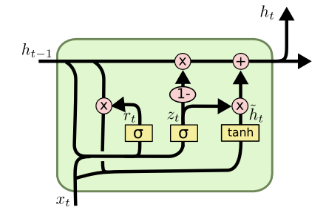
\includegraphics[width=0.8\textwidth]{pic/12.PNG}
\end{minipage}
%
\begin{minipage}[c]{0.5\textwidth}
\begin{equation*}
	\begin{array}{l}
	z_t = \delta(W_z \cdot [h_{t-1}, x_t]) \\
	r_t = \delta(W_r \cdot [h_{t-1}, x_t]) \\
	\tilde{h}_{t} = \tanh(W \cdot [r_t * h_{t-1}, x_{t}])\\
	h_t = (1-z_t) * h_{t-1} + z_t * \tilde{h}_t \\
	\end{array}
\end{equation*}
\end{minipage}
\label{fig:12} 
\caption{Variant of LSTM 3: Gated Recurrent Unit, GRU}
\end{figure}

%\bibliographystyle{plain}
\bibliographystyle{unsrt}
\bibliography{reference}
\end{document}